\setcounter {section} {0}
\section{Phase 1 - Level 2: The Queues Manager}

Level 2 of JaeOS instantiates the key operating system concept that active entities at one layer are just data structures at lower layers. 
In this case, the active entities at a higher level are processes (i.e. programs in execution) and the data structure(s) that represent them at this level are process control blocks (ProcBlk’s).

The queue manager will implement four ProcBlk related functions:
\begin{itemize}
	\item The allocation and deallocation of ProcBlk’s.
	\item The maintenance of queues of ProcBlk’s.
	\item The maintenance of trees of ProcBlk’s.
	\item The maintenance of a single sorted list of active semaphore descriptors each of which supports a queue of ProcBlk’s.
\end{itemize}

\noindent
\begin{lstlisting}
struct semd_t;
/* process control block type */
struct pcb_t {
    struct pcb_t *p_parent; /* pointer to parent */
    struct semd_t *p_cursem; /* pointer to the semd_t on
				which process blocked */
    state_t p_s; /* processor state */
    struct clist p_list; /* process list */
    struct clist p_children; /* children list entry point*/
    struct clist p_siblings; /* children list: links to the 
    				siblings */
};
\end{lstlisting}

\subsection{The Allocation and Deallocation of ProcBlk’s}

One may assume that JaeOS supports no more that MAXPROC concurrent processes; where MAXPROC should be set to 20 (in the file CONST.H).

Thus this level needs a pool of MAXPROC ProcBlk’s to allocate from and deallocate to. 
Assuming that there is a set of MAXPROC ProcBlk’s, the free or unused ones can be kept on a list pointed to by the variable pcbFree (of type \verb+struct clist+).

To support the allocation and deallocation of ProcBlk’s there should be the following three externally visible functions:
\begin{itemize}
	\item ProcBlk’s which are no longer in use can be returned to the pcbFree list by using the method:\\
		\verb+void freePcb(struct pcb_t *p)+\\
		insert the element pointed to by p onto the pcbFree list.
	\item ProcBlk’s should be allocated by using:\\
		\verb+struct pcb_t *allocPcb()+\\
		Return NULL if the pcbFree list is empty. Otherwise, remove an element from the pcbFree list, provide initial values for ALL of the ProcBlk’s fields (i.e. fill the entire structure by NULL/zero bytes) and then return a pointer to the removed element. ProcBlk’s get reused, so it is important that no previous value persist in a ProcBlk when it gets reallocated. 
		There is still the question of how one acquires storage for MAXPROC ProcBlk’s and gets these MAXPROC ProcBlk’s initially onto the pcbFree list. 
		Unfortunately, there is no malloc() feature to acquire dynamic (i.e. non-automatic) storage that will persist for the lifetime of the OS and not just the lifetime of the function they are declared in. 
		Instead, the storage for the MAXPROC ProcBlk’s will be allocated as static storage. 
		A static array of MAXPROC ProcBlk’s will be declared in initPcbs(). 
		Furthermore, this method will insert each of the MAXPROC ProcBlk’s onto the pcbFree list.
	\item To initialize the pcbFree List:\\
		\verb+void initPcbs(void)+\\
		Initialize the pcbFree list to contain all the elements of the static array of MAXPROC ProcBlk’s. This method will be called only once during data structure initialization.
\end{itemize}

\subsection{Process Queue Maintenance}

\begin{figure}[htbp]
	\centering
	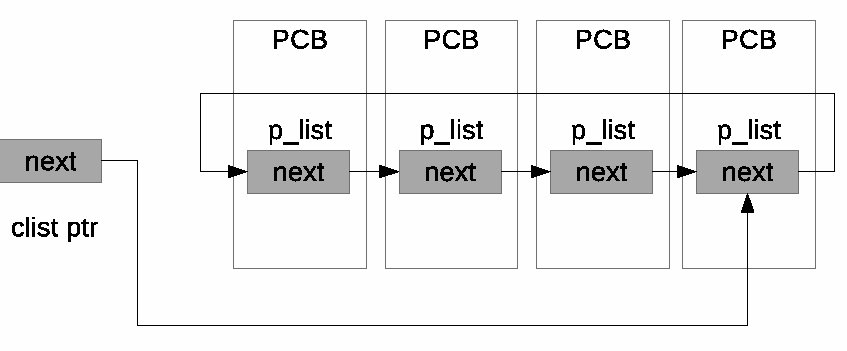
\includegraphics[width=.9\textwidth]{\docsd/graphs/queue.png}
	\caption*{}
\end{figure}

The methods below do not manipulate a particular queue or set of queues.
Instead they are generic queue manipulation methods; one of the parameters is a pointer to the queue upon which the indicated operation is to be performed.

A new process queue is a Linux kernel list (implemented through the macros and inline functions of \verb+listc.h+) thus it can be created using either the macro \verb+LIST_HEAD_INIT+ or the inline function \verb+INIT_LIST_HEAD+.
It is possible to test if a process queue is empty using the \verb+list_empty+ inline function provided in \verb+listx.h+.

To support process queues there should be the following externally visible functions:
\begin{itemize}
	\item \verb+void insertProcQ(struct clist *q, struct pcb_t *p)+\\
		Insert the ProcBlk pointed to by p into the process queue whose list-tail pointer is q.
	\item \verb+struct pcb_t *removeProcQ(struct clist *q)+\\
		Remove the first (i.e. head) element from the process queue whose list tail pointer is q. Return NULL if the process queue was initially empty; otherwise return the pointer to the removed element.
	\item \verb+struct pcb_t *outProcQ(struct clist *q, struct pcb_t *p)+\\
		Remove the ProcBlk pointed to by p from the process queue whose list-tail pointer is q. 
		If the desired entry is not in the indicated queue (an error condition), return NULL; otherwise, return p. Note that p can point to any element of the process queue.
	\item \verb+struct pcb_t *headProcQ(struct clist *q)+\\
		Return a pointer to the first ProcBlk from the process queue whose list-tail pointer is q. 
		Do not remove this ProcBlk from the process queue.
		Return NULL if the process queue is empty.
\end{itemize}

\subsection{Process Tree Maintenance}

\begin{figure}[htbp]
	\centering
	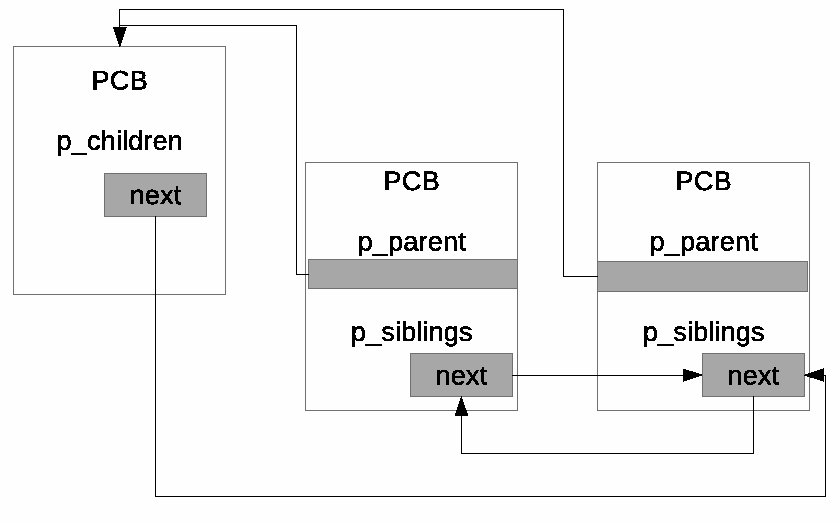
\includegraphics[width=.9\textwidth]{\docsd/graphs/tree.png}
	\caption*{}
\end{figure}

In addition to possibly participating in a process queue, ProcBlk’s are also organized into trees of ProcBlk’s, called process trees. 
The \verb+p_childred+, \verb+p_siblings+ and \verb+p_parent+ fields of the \verb+struct pcb_t+ are used for this purpose. 
\verb+p_childred+ is the entry point of the list of all the children of the process, linked together using the \verb+p_siblings+ field.
Each child process has a pointer to its parent ProcBlk (\verb+p_parent+).
To support process trees there should be the following externally visible functions:
\begin{itemize}
	\item \verb+int emptyChild(struct pcb_t *p)+\\
		Return TRUE if the ProcBlk pointed to by p has no children. 
		Return FALSE otherwise.
	\item \verb+void insertChild(struct pcb_t *parent, struct pcb_t *p)+\\
		Make the ProcBlk pointed to by p a child of the ProcBlk pointed to by parent.
	\item \verb+struct pcb_t *removeChild(struct pcb_t *p)+\\
		Make the first child of the ProcBlk pointed to by p no longer a child of p.
		Return NULL if initially there were no children of p. 
		Otherwise, return pointer to this removed first child ProcBlk.
	\item \verb+struct pcb_t *outChild(struct pcb_t *p)+\\
		Make the ProcBlk pointed to by p no longer the child of its parent. 
		If the ProcBlk pointed to by p has no parent, return NULL; otherwise, return p. 
		Note that the element pointed to by p need not be the first child of its parent.
\end{itemize}

\subsection{The Active Semaphore List}

\begin{figure}[htbp]
	\centering
	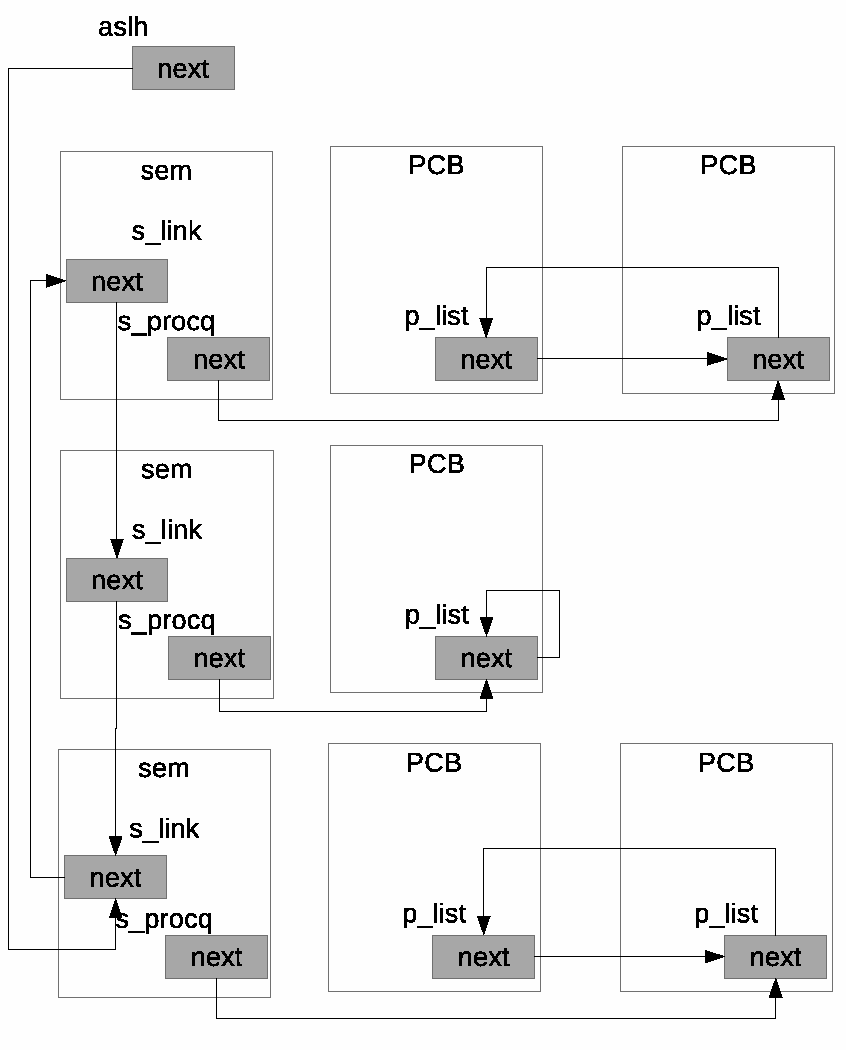
\includegraphics[width=.9\textwidth]{\docsd/graphs/asl.png}
	\caption*{}
\end{figure}

A semaphore is an important operating system concept which is needed for Phase 2/Level 3. 
While understanding semaphores is not needed for this level, this level nevertheless implements an important data structure/abstraction which supports JaeOS’s implementation of semaphores. 
For the purposes of this level it is sufficient to think of a semaphore as an integer. 
Associated with this integer is its address (semaphores, like all integers, have a physical address) and a process queue. 
A semaphore is active if there is at least one ProcBlk on the process queue associated it. 
The following implementation is suggested: maintain a sorted list of semaphore descriptors. 
This list represents the Active Semaphore List (ASL). Its entry point is the variable named \verb+aslh+ (of type \verb+struct clist+). 
Keep the ASL sorted in ascending order using the address of the semaphore (\verb+s_semAdd+ field) as the sort key.

Maintain a second list of semaphore descriptors, the semdFree list, to hold the unused semaphore descriptors. 
The semaphore descriptors themselves should be declared, like the ProcBlk’s, as a static array of size MAXPROC of type \verb+{struct semd_t}.+

\begin{lstlisting}
struct semd_t {
    int *s_semAdd; /* pointer to the semaphore */
    struct clist s_link; /* ASL linked list */
    struct clist s_procq; /* blocked process queue */
};
\end{lstlisting}

To support the ASL there should be the following externally visible functions:
\begin{itemize}
	\item \verb+int insertBlocked(int *semAdd, struct pcb_t *p)+\\
		Insert the ProcBlk pointed to by p at the tail of the process queue associated with the semaphore whose physical address is semAdd and set the semaphore address of p to semAdd. 
		If the semaphore is currently not active (i.e. there is no descriptor for it in the ASL), allocate a new descriptor from the semdFree list, insert it in the ASL (at the appropriate position), initialize all of the fields (i.e. set \verb+s_semAdd+ to \verb+semAdd+, and \verb+s_procq+), and proceed as above. 
		If a new semaphore descriptor needs to be allocated and the semdFree list is empty, return TRUE. In all other cases return FALSE.
	\item \verb+struct pcb_t *removeBlocked(int *semAdd)+\\
		Search the ASL for a descriptor of this semaphore. 
		If none is found, return NULL; otherwise, remove the first (i.e. head) ProcBlk from the process queue of the found semaphore descriptor and return a pointer to it. 
		If the process queue for this semaphore becomes empty remove the semaphore descriptor from the ASL and return it to the semdFree list.
	\item \verb+struct pcb_t *outBlocked(struct pcb_t *p)+\\
		Remove the ProcBlk pointed to by p from the process queue associated with p’s semaphore on the ASL.
		If ProcBlk pointed to by p does not appear in the process queue associated with p’s semaphore, which is an error condition, return NULL; otherwise, return p. 
	\item \verb+struct pcb_t *headBlocked(int *semAdd)+\\
		Return a pointer to the ProcBlk that is at the head of the process queue associated with the semaphore semAdd. 
		Return NULL if semAdd is not found on the ASL or if the process queue associated with semAdd is empty.
	\item \verb+void initASL(void)+\\
		Initialize the semdFree list to contain all the elements of the array \\
		\verb+static struct semd_t semdTable[MAXPROC]+\\
		This method will be only called once during data structure in initialization.
\end{itemize}

\subsection{Nuts and Bolts}
There is no one right way to implement the functionality of this level. 
One approach is to create two modules: one for the ASL and one for ProcBlk initialization/allocation/deallocation, process queue maintenance, and process tree maintenance.

The second module, PCB.C, in addition to the public and HIDDEN/private (static) helper functions, will also contain the declaration for the private global variable that points to the head of the pcbFree list, e.g.\\
\verb+HIDDEN struct clist pcbFree;+

The ASL module, ASL.C, in addition to the public and HIDDEN/private helper functions, will also contain the declarations for aslh and semdFree, e.g.\\
\verb+HIDDEN struct clist aslh, semdFree;+

Since the ASL module will make calls to the process queue module to manipulate the process queue associated with each active semaphore, this module should \verb+#include+ \verb+"pcb.h"+.
This will insure that the ASL can only use the externally visible functions from PCB.C. for maintaining its process queues.
Furthermore, the declaration for \verb+struct pcb_t+ would then be placed in \verb+types.h+.
This is because many other modules will need to access this definition. 
The declaration for \verb+struct semd_t+ is placed in ASL.C because no other module will ever need to access this definition; hence it is local to the module. 
As with any non-trivial system, you are strongly encouraged to use the make program to maintain your code.

\subsection{Testing}
There will be a provided test file, P1TEST.C that will exercise your code.
The test program reports on its progress by writing messages to TERMINAL0.
These messages are also added to one of two memory buffers; errbuf for error messages and okbuf for all other messages. 
At the conclusion of the test program, either successful or unsuccessful, arm will display a final message. 
The final message will either be SYSTEM HALTED for successful termination, or KERNEL PANIC for unsuccessful termination.


